\section{Overview}

In this experiment the influence of tube voltage and resolving time on
the counting efficiency of a Geiger-Muller tube are explored. \ The
tube is then used to study a simple radioactive decay and a
parent-daughter system.

\section{Theory}

\subsection{Geiger-Muller Tube Characteristics}
\label{sec:GMtubes}

A Geiger-Muller (or G-M) tube is a simple device to detect energetic
particles (or photons) emitted as
``radiation''.  Such radiation can arise
from a variety of sources, the most common being the decay of unstable
(or ``radioactive'') nuclei. A G-M tube is
typically a cylindrical gas-filled chamber sealed at one end by a thin
sheet or ``window'' (often made of mica)
through which energetic particles and photons can pass. A wire running
down the center of the chamber is kept at a positive voltage relative
to the chamber wall.

Upon entering the chamber, the radiation particle collides with gas
molecules causing ionization - the removal of electrons from some
molecules leaving them as positively charged ions.  The voltage
between the wall of the tube and the central wire causes the ions and
freed electrons to move, leading to further collisions and more
ionization.  In a short time, enough ions and electrons are present to
allow an electric current pulse to flow between the wall and wire.
 This pulse is recorded by a counter (or
``scalar''). The flow of the current pulse
leads to the neutralization of the
gas ions in the tube and, after a short time (known as the
``resolving time'') the tube is able to
respond again to an incoming particle.

The performance of a G-M tube depends on the tube voltage (applied
between the center wire and the wall).  If this voltage is too small,
insufficient ionization occurs to register a count on the scalar.  If
the voltage is too large, a continuous discharge current occurs, which
damages the tube.  As the voltage is increased gradually, the counting
rate increases steadily until a threshold is reached, followed by a
``plateau'' region in which the counting rate
is approximately constant.  Following the
plateau, further increases in tube voltage lead to rapid increases in
counts and one begins to enter the continuous discharge region.  In
practice, a G-M tube should be operated in the plateau region.  This
protects the tube and ensures that uncontrollable fluctuations in tube
voltage will not significantly affect the count data.


We have seen that a process of detection of a particle in a G-M tube
requires a certain amount of time (called the resolving time). If a
second particle enters the tube during this time (while ionization and
current flow from the first particle are taking place), it will not be
recorded as a separate count.  Thus, the actual counting rate is
higher than that measured by the tube and, for precise work, a
correction must be applied.  The correction can be derived as follows.

Suppose $n$ counts are recorded on the scalar in time $t$.  Then the
measured counting rate $R~=~n/t$.  Let us denote the resolving time by
$t_r$.  Then for each particle counted the tube
was unavailable for a time $t_r$, so that during the
counting time $t$, the tube was actually available to record particles
only for a time equal to $t - n t_r$ . Thus, the corrected
counting rate $R_{c}$ is given by number of counts divided by the {\em available} counting time, or
\begin{equation}
R_c ~=~ { n \over t - n t_r }
\label{eq:1}
\end{equation}
Dividing numerator and denominator of the last expression in Eq.~\ref{eq:1} by
$t$, one obtains
\begin{equation}
R_c ~=~ { R \over 1 - R t_r }
\label{eq:2}
\end{equation}
For typical counting rates, $R t_{r} \ll 1$, and therefore Eq.~\ref{eq:2} can be approximated,
using the binomial expansion on $(1-R t_r)^{-1}$, as
\begin{equation}
R_{c} \approx R(1 + Rt_{r}) = R + (Rt_{r})(R)
\label{eq:3}
\end{equation}

Thus, the correction added to $R$ is expressed as a fraction of $R$, the
fraction being equal to $Rt_{r}$.  The relative
magnitude of the correction increases as $R$ increases, which is to be
expected, since for higher count rates the tube will
``miss'' relatively more counts.
Physically, the approximation
$Rt_{r} \ll 1$ means that the resolving
time $t_{r}$ is much shorter than the average time between
counts $1/R$.  This approximation will break down for sufficiently high
count rates.

How is the resolving time determined?  A simple method to be carried
out in this experiment involves measuring the counting rate for two
sources together and individually - always keeping the each source in
the same position relative to the tube when it is being measured.  Let
$R_{1}$ and $R_{2}$ be the measured counting
rates when sources 1 and 2 are measured individually, and let
$R_{b}$ be the measured counting rate when both sources are
present. We know that $R_{bc} ~=~ R_{1c} + R_{2c }$,
since sources 1 and 2 decay independently of one
another.  However, due to the resolving time effect, we expect that
$R_{b} < R_{1} + R_{2}$, since at the higher counting rate which occurs when both sources are
present, a greater fraction of counts will be lost.  Applying  Eq.~\ref{eq:3}
to this situation, one can show that the resolving time may be
(approximately) found from
\begin{equation}
t_r ~=~ { R_1 + R_2 - R_b \over 2 R_1 R_2 }
\label{eq:4}
\end{equation}
Similar approximations are made in deriving Eq.~\ref{eq:4} as were used in
obtaining Eq.~\ref{eq:3} from Eq.~\ref{eq:2}.  Typical resolving times for G-M tubes
are hundreds of microseconds.

\subsection{Radioactive Decay}
\label{sec:rad-decay}

In a sample containing $N$ identical unstable nuclei it is found
experimentally that the number of nuclei decaying in a short time $dt$ is
proportional to $N dt$.  Since this number equals the decrease $-dN$
in the number of nuclei present, we can write
\begin{equation}
- {dN \over dt} ~=~ -K N dt
\label{eq:5}
\end{equation}
where $K$ is a proportionality constant, known as the decay constant.
Rearranging Eq.~\ref{eq:5}, we obtain the differential equation
\begin{equation}
{dN \over dt} ~=~ -K N
\label{eq:6}
\end{equation}

Note that $N$ is the number of undecayed nuclei, and will decrease as time
t increases.  $dN/dt$ is the rate of change of $N$ and is a negative
quantity.  Its absolute value gives the decay rate (number of decays
per unit time) at any given time.  This quantity is often called the
``activity'' of the sample and will be denoted by $A$.  Hence we have
\begin{equation}
A ~=~ - { dN \over dt } ~=~ KN
\label{eq:7}
\end{equation}
so that the activity is directly proportional to the number of nuclei
remaining.  The differential equation~\ref{eq:6} has the solution
\begin{equation}
N = N_{0} e^{-Kt}
\label{eq:8}
\end{equation}
where $N_0$ is the number of unstable nuclei present at time $t~=~0$ and $N$ is
the number remaining at time $t$.  Eq.~\ref{eq:8} gives the familiar decreasing
exponential behavior associated with radioactive decay.  Since the
activity $A$ is directly proportional to $N$, $A$ will obey the same
exponential decay law as $N$.

The activity itself is not measured with our apparatus, since only a
fraction of the decaying particles travel in a direction which allows
them to enter the G-M tube window.  However, if the radioactive sample
and tube are not moved during measurement and if conditions affecting
the tube performance are constant, then the observed count rate $R$ will be some
definite fraction of $A$ and hence will also obey the exponential decay
law
\begin{equation}
R = R_{o} e^{-Kt}
\label{eq:9}
\end{equation}
We can determine the decay constant $K$ from a semi-log plot of the
measured count rate {\em vs.} time.

The ``half-life'' T is defined as the time
required for 1/2 of the nuclei present at any given time to decay.
For example, if there are $N_0$ nuclei present at time $t = 0$, then at
time $t = T$ the number $N$ remaining will be $N_0/2$.  In this situation,
Eq.~\ref{eq:8} allows us to find an expression for $T$ as follows:  

\begin{eqnarray}
N ~=~ {N_0 \over 2} &=& N_0 e^{-KT}\\
 {1 \over 2} &=& e^{-KT}
\end{eqnarray}
from which it follows that the half-life T is given by
\begin{equation}
T ~=~ {\ln{2} \over K} = {0.693 \over K}
\label{eq:11}
\end{equation}

\subsection{Parent-Daughter Systems}
\label{sec:parent-daughter}

It often happens that the residual nucleus left after the decay of a
radioactive nucleus is also radioactive.  In this case, the original
nucleus is called the parent and the residual nucleus the daughter.
Assume that the parent nuclei decay according to the relation

\begin{equation}
N ~=~ N_0 e^{-Kt}
\label{eq:12}
\end{equation}

The rate of change of the number of daughter nuclei present will equal
the rate of parent decay minus the rate of daughter decay.  If the
number of daughter nuclei is denoted by $N^\prime$ and the
corresponding decay constant by $K^\prime$, then we have

\begin{equation}
{dN^\prime \over dt} ~=~ KN - K^\prime N^\prime
\label{eq:13}
\end{equation}

Combining Eqs.~\ref{eq:12} and \ref{eq:13}, one can arrive at a general solution for
$N^\prime$ as a function of time $t$.
An interesting special case is that for which
$T^\prime \ll T$, i.e. the daughter decays
much more rapidly than the parent. If one begins with a source
containing only parent nuclei and no daughters present, then the
number of daughter grows gradually toward a steady
state value $N^\prime$ at which the rates of decay (or
activities) of the parent and daughter are equal.  Under these
conditions we have

\begin{eqnarray}
A_{\rm parent} ~=~ A_{\rm daughter} \\
KN = K^\prime N^\prime
\label{eq:14}
\end{eqnarray}

In our experiment we measure the sum of the parent and daughter count
rates.  The time of measurement is comparable to the daughter
half-life and much shorter than the parent half-life.  At time $t = 0$,
we have a count rate of $R_0$ which is entirely due to
parent nuclei decays, since (by assumption) no daughter nuclei are
present at $t = 0$.  By the end of the experiment, steady state is reached.
The count rate for the parent is still close
to $R_0$ (why?) while the daughter rate is equal to that
of the parent.  Hence, in steady state, the total measured count rate
is expected to be about $2R_0$, twice as large as at $t = 0$.

Knowing $K$ and $K^\prime$, Eq.~\ref{eq:14} allows one to calculate the
parent-daughter ratio $N/N^\prime$ in steady state.  This
makes it possible to compute the relative abundances of nuclei in a
radioactive decay chain.

\section{Preliminary Questions}

\begin{enumerate}
\item For \cs, the accepted value for the half-life is 30.1 years,
while for \bam, the half-life = 2.6 minutes.  Assume that in a \cs-\bam generator,
the parent (\cs) and daughter (\bam) are in a steady state
situation---which will be the case if no daughter nuclei have been
removed within the last hour. Use Eqs~\ref{eq:11} and \ref{eq:14} to calculate the
ratio $N^\prime/N$ of daughter to parent nuclei in the
generator.

\item ({\em Optional}: 1 point extra credit.) Derive Eq.~\ref{eq:4} for the
resolving time $t_r$ of a G-M tube, starting from the fact
that $R_{bc } ~=~  R_{1c } + R_{2c }$.  Use Eq.~\ref{eq:3} and the approximation
$Rt_{r} \ll 1$ (where $R$ can be $R_{1}$, $R_{2}$ or $R_{b}$).

{\em Note}: Please do not spend more than 1 hour on this question.  Carrying
through the calculation while consistently applying the approximations
involved is not entirely straightforward.
\end{enumerate}

\section{Equipment}
Geiger-Muller tube, scalar, sample holder, planchets,
sealed radioactive sources, \cs --- \bam generator.

\bigskip

{\bf CAUTION: DO NOT HANDLE ANY OF THE RADIOACTIVE SOURCES.}

Notify the instructor immediately in the event of a spill of a radioactive
solution or any other accident.  The instructor will perform elutions
and place solutions in the sample holder.  Rubber gloves ,ust be worn
when working with liquid radioactive sources.


\section{Procedure}

\begin{enumerate}
\item A long half-life source, ${}^{204}{\rm Tl}$, will be placed in the sample
holder.  This isotope of Thallium emits $\beta^-$ (electrons) with an energy of 0.764 MeV.  Starting with the tube voltage at its lowest setting, count
for brief periods, increasing the voltage until you first begin
observing decays.  No quantitative data is needed at this stage.
What can you say about the tube when no decays are obtained?

\item Once the tube voltage is sufficient to produce decays, record the
number of counts in a short time interval (say 10 seconds --- assuming one obtains at least
several hundred counts during that time) for values of voltage varied
by increments of 40 volts.  Do not exceed the maximum voltage
specified by your instructor, about 1000 V for the B210 tubes we are using.

As the tube voltage is increased, you should find that the number of
counts in the time interval increases rapidly at first, then goes
through a stage where the number of counts is nearly constant (the
``plateau'' region).  When the voltage is
further increased, the number of counts begins to increase very
rapidly.
\begin{figure}
\begin{centering}
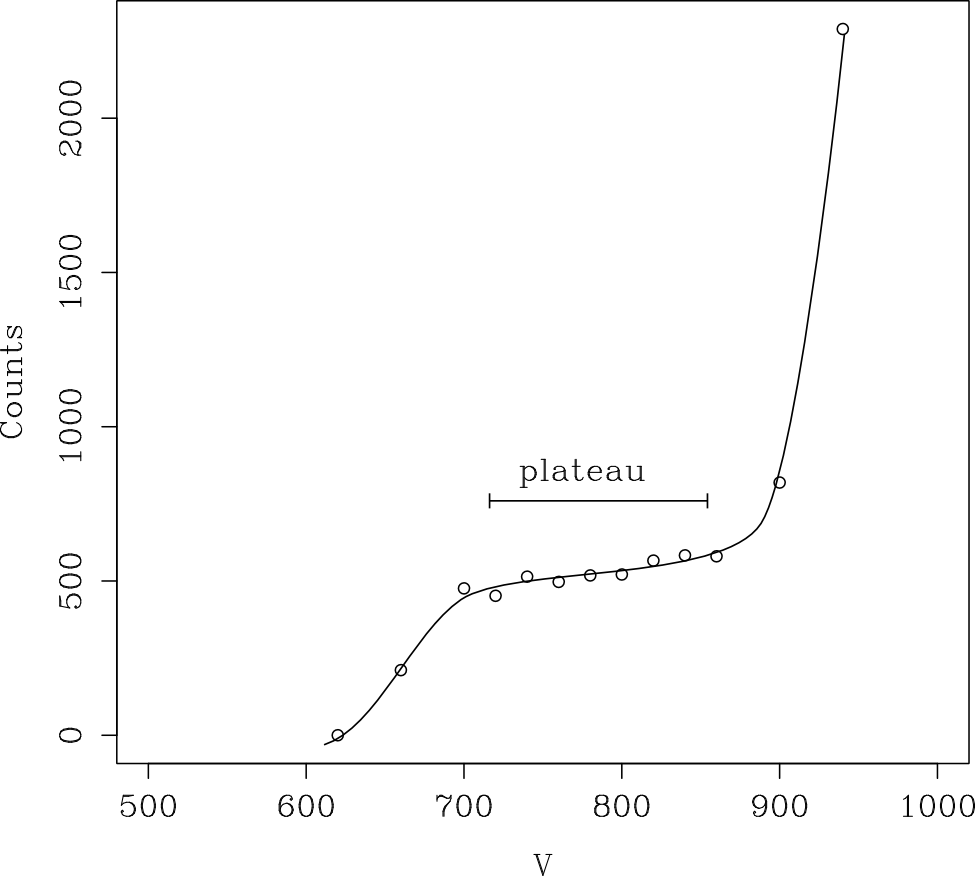
\includegraphics[width=4in]{../images/gmplateau.png}
\caption{Student data showing the plateau region of the counts vs. voltage plot for a B210/BNC Geiger-Muller Tube.}
\label{fig:rate-V}
\end{centering}
\end{figure}
A sample of student data is shown in Figure~\ref{fig:rate-V}.

\item Sketch a graph of counts vs. tube voltage and find the
plateau region.  Take a few more readings as in step 2 for voltages in
the plateau region.  Choose an optimum operating tube voltage---where
the number of counts is as close as possible to being constant for
voltages near this optimum value. Keep the tube voltage set at this
value throughout the remainder of the experiment.

\item To determine the resolving time of your G-M tube, measure the count
rate for three configurations: first, source 1 present; second, both 1
and 2 present; and third, only 2 present.  The instructor will change
the configurations, keeping the sample locations fixed when they are
being measured.  Use a one-minute counting time, and measure each
configuration four times.  Sources 1 and 2 are ${}^{204}{\rm Tl}$.

{\em Note}: Before going on, perform the following check on your data.
Assume that the resolving time $t_{r}$ of your G-M tube is
300 microseconds $ = 3 \times 10^{-4}$ seconds.  Evaluate the
quantity $R_{b} t_{r}$ numerically. Show your results
to your instructor. Does the relation
$ R_{b} t_{r} \ll 1$ hold ?
If so, you may go on to the rest of the experiment.  If not, you
must repeat the measurements in this step and place the radioactive
sources farther from the G-M tube.  It is important that all count
rates are small enough so that $R_{b}t_{r} \ll 1$, since our treatment of resolving time
assumes $R_{b}t_{r} \ll 1$.

\item With no sources in the sample holder or nearby, measure the
background count rate.  Use a one-minute interval and take four
measurements.  The average background count rate must be subtracted
from all count rate data taken on particular sources.

\item The instructor will elute a solution through the generator
containing the parent nuclei \cs and daughter nuclei \bam.  The
\bam nuclei are transported as ions in the solution out of the
generator.  The instructor will put this solution into a planchet (a
small metal dish) and place it in the sample holder.  Immediately
begin to measure the count rate of the \bam source.  Use 10 second
intervals, with each interval starting one
minute after the start of the previous interval.  Continue for a total
of 20 minutes---or until the count rate no longer varies significantly
from one reading to the next. 

\item The instructor will elute a solution through the \cs generator,
put the solution aside, and place the generator itself in the sample
holder. This approximates an initial situation with parent and no
daughter present. Begin counting immediately, using the same timing as
in the previous step.  Continue for 20 minutes---or until the count
rate no longer varies significantly from one reading to the next.
\end{enumerate}

\section{Analysis}

\begin{enumerate}
\item Make a careful plot of your count vs. tube voltage data.
Indicate on your graph the plateau and the operating voltage used in
your experiment.

\item Compute the resolving time of the G-M tube using averaged count
rates from Procedure step 4.

\item Correct the \bam count rate data (from Procedure step 6), first
for background and then for resolving time (see Eq.~\ref{eq:3}).  Then plot
the corrected count rate $R_{c}$ vs. time on
Cartesian and semi-log axes.  Describe the shape of the two graphs
and discuss what this shape indicates about the mathematical
relationship between $R_{c}$ and $t$.
\begin{figure}
\begin{centering}
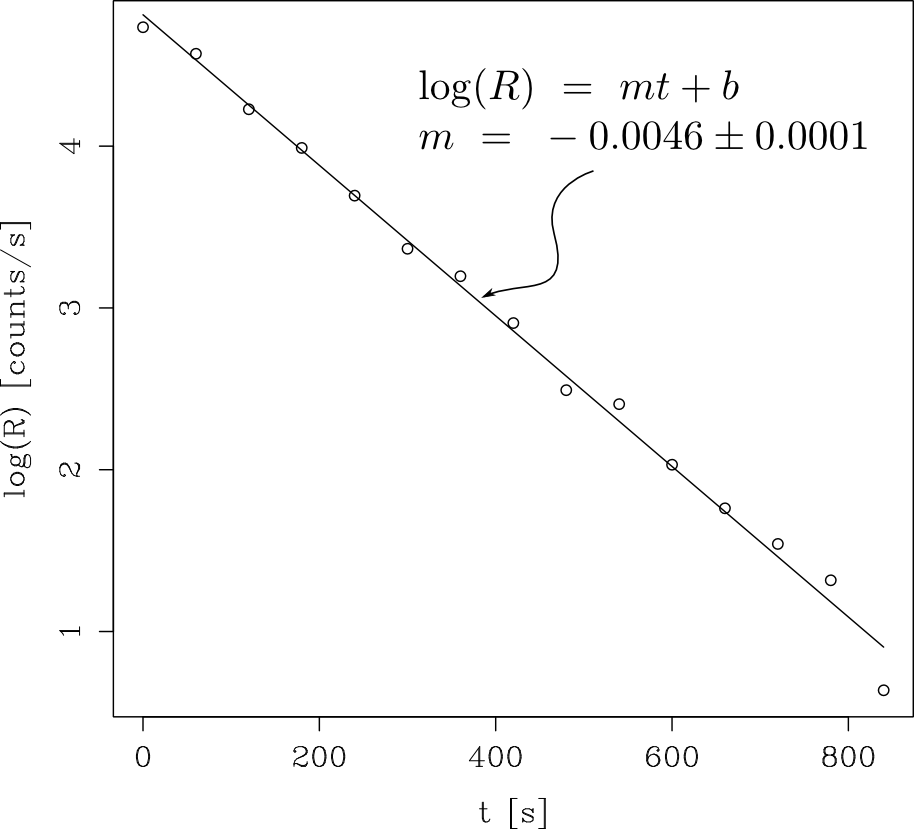
\includegraphics[width=4in]{../images/ba137m.png}
\caption{Example of student data showing the $\log(R_c)$ vs. time for the \bam data.  The straight line fit yields a slope of $m=-0.0046\pm0.0001$, corresponding to a \bam half-life of $2.511\pm0.054$ m. }
\label{fig:rate-V}
\end{centering}
\end{figure}

{\em Note}: All count rates must be in the same units, e.g. counts/minute. 
It may occur that for the last data points, the corrected count
rates might be slightly negative.  Those points must be eliminated
from the data in order to do the required data analysis.

\item Perform an appropriate curve fit on the $R_{c}$ vs. $t$ data
from Procedure step 6, and obtain the decay
constant $K$. Then compute the half-life $T$ of \bam.  Find the
uncertainty in the decay constant $K$ by applying the Excel function
{\tt LINEST} to the decay data in the form $\ln(R_{c})$ as a
function of $t$.  The accepted value of the half-life $T$ of \bam is
given in Preliminary Question 1. Compare it to the measured value of $T$,
taking the uncertainty into account.

{\em Note}: If {\tt LINEST} is not available, use the $\ln(R_{c})$ versus
$t$  graph and perform ``by hand'' another
curve fit.  The difference in slopes for the two fits (one done by
Excel and the other by hand) is a rough measure of the uncertainty in
the slope and hence, the uncertainty in $K$.

\item On your Cartesian graph of corrected count rate vs. time
for \bam, choose two points separated in time by one half-life (as
determined in step 4 above).  What should the ratio of the count rates
at those two points be?  Compare to the ratio obtained from the points
on your graph.

\item Correct the \bam count rate data for background and for
resolving time. Plot the count rate vs. time for the
parent-daughter system (on Cartesian axes).  Explain in your own words
the shape of this graph.  Consider the initial and final values of the
count rate.  What should the ratio of the final to the initial count
rates be, according to theory?  How do your results compare to the
theoretical prediction?
\end{enumerate}

\section{References}
\begin{enumerate}
\item Thornton and Rex, Modern Physics, $3^{\rm rd}$ ed., pp. 441-444
\item Tipler and Llewellyn, Modern Physics, $5^{\rm th}$ ed., pp. 492-494
\end{enumerate}
